% Part: history
% Chapter: set-theory
% Section: limits

\documentclass[../../../include/open-logic-section]{subfiles}

\begin{document}
	
\olfileid{his}{set}{limits}	

\olsection{పరిమితుల కచ్చిత నిర్వచనం}
	
ఈ రోజుల్లో ముందరి సమస్యకు ప్రామాణిక పరిష్కారం అనంతసూక్ష్మాలను వదిలేయడమే. అది ఎలా సాధ్యమో చూద్దాం.

$\beta$ చిన్నదవుతున్న కొద్దీ వాలుకు మెరుగైన ఉజ్జాయింపులు వస్తాయని చూశాం. నిజానికి $\beta$ విలువ $0$కు ఎంత దగ్గరగా కావాలంటే అంత దగ్గరగా వెళ్లినప్పుడు, భేద భాగహారం విలువ మనకు కావలసిన వాలు $f'(c)$ వైపు చేరుతుంది. కనుక $\beta = 0$ \emph{వద్ద} ఏమవుతుందో పరిశీలించకుండా, $\beta$ అనేది $0$కు చేరుతున్నప్పుడు $f'(c)$ను ఇచ్చే ఆ భాగహారం యొక్క \emph{ధోరణి}ని పరిశీలిస్తే చాలు.
\sourcecorrection{OLTEHISSETLIM-001}{మూలం బీటా మారుతున్నప్పుడు స్థిర బిందువులోని వ్యుత్పన్న విలువే మారుతున్నట్లు చెప్పింది; మారేది భేద భాగహారం విలువ. ఆ భావాన్ని స్పష్టంగా సరిచేశాం.}

సాధారణంగా చెప్పాలంటే, ఇలాంటి వాదనలకు అర్థం ఇవ్వడమే మన ముందున్న పని:
\begin{center}
$x$ అనేది $c$కు చేరుతున్నప్పుడు, $g(x)$ అనేది $\ell$ వైపు చేరుతుంది.
\end{center}
దీన్ని మరింత సంక్షిప్తంగా ఇలా రాయవచ్చు:
\[
\lim_{x \rightarrow c}g(x) = \ell.
\]
పంతొమ్మిదో శతాబ్దంలో కౌషీ పూర్వ కృషిపై ఆధారపడి, వైయర్‌స్ట్రాస్ ఈ వ్యక్తీకరణకు పూర్తిగా కచ్చితమైన నిర్వచనం ఇచ్చారు. $x$ను $c$కు తగినంత దగ్గరగా తీసుకోవడం ద్వారా $g(x)$ను~$\ell$కు మనం కోరుకున్నంత దగ్గరగా తీసుకురాగలమన్నదే ఆ భావం. ఇంకా కచ్చితంగా, $\lim_{x \rightarrow c} g(x) = \ell$ అంటే ఇలా అని నిర్ణయిస్తాం:
\[
(\forall\epsilon > 0)(\exists \delta > 0)\forall x \left(0<|x - c| < \delta \lif |g(x) - \ell| < \epsilon \right).
\]
\sourcecorrection{OLTEHISSETLIM-002}{మూల పరిమితి నిర్వచనం కేంద్ర బిందువును కూడా పూర్వపక్షంలో చేర్చింది. సాధారణ పరిమితికి కేంద్రంలో ప్రమేయం విలువ అవసరం లేదు; అందుకే శూన్యం కంటే కచ్చితంగా ఎక్కువ దూరం అనే షరతును చేర్చాం.}
ఇక్కడ నిలువు గీతలు పరమ విలువను సూచిస్తాయి. అంటే $x \geq 0$ అయితే $|x| = x$; $x < 0$ అయితే $|x| =-x$; \emph{ఆ} ప్రమేయాన్ని ఇలా చిత్రించవచ్చు:
\begin{center}
	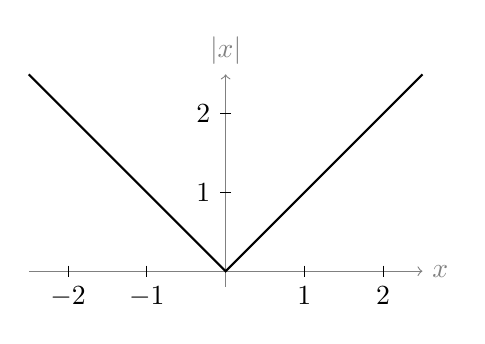
\begin{tikzpicture}[scale=1]
	\draw[->, gray] (-2.5,0) -- (2.5,0) node[right] {$x$};
	\draw[->, gray] (0,-.2) -- (0,2.5) node[above] {$|x|$};
	
	\foreach \x/\xtext in {-2/-2, -1/-1, 1/1, 2/2}
	\draw[shift={(\x,0)}] (0pt,2pt) -- (0pt,-2pt) node[below] {{$\xtext$}};
	
	\foreach \y/\ytext in {1/1, 2/2}
	\draw[shift={(0,\y)}] (2pt,0pt) -- (-2pt,0pt) node[left] {{$\ytext$}};
	
	\draw[thick] (-2.5, 2.5)--(0,0)--(2.5, 2.5);
	\end{tikzpicture}
\end{center}
\sourcecorrection{OLTEHISSETLIM-003}{మూల చిత్రపు అడ్డ అక్షం గుర్తుల జాబితాలో రుణ ఒకటి దగ్గర జత చిహ్నం లేకుండా అదనపు ఒకటి ఉంది; రుణ రెండు, రుణ ఒకటి, ఒకటి, రెండు గుర్తులు ఒక్కొక్కటే వచ్చేలా చేశాం.}
కాబట్టి ఈ నిర్వచనం స్థూలంగా ఇలా చెబుతుంది: $c$ నుంచి $\delta$ కంటే తక్కువ దూరంలో ఉన్న ఆర్గ్యుమెంట్లను ఎంచుకోవడం ద్వారా (అంటే $|x -
c| < \delta$), మీ ``దోషం'' $\epsilon$ కంటే తక్కువగా (అంటే $|g(x) - \ell| < \epsilon$) చేయవచ్చు.

పరిమితి భావనను నిర్వచించాం కనుక, అనంతసూక్ష్మాలను పూర్తిగా వదిలేసి $c$ వద్ద $f$ వాలు ఇలా వస్తుందని నిర్ణయించవచ్చు:
\[
	{f}'(c) = \lim_{x \rightarrow 0}\left(\frac{f(c +x) - f(c)}{x}\right) \text{ పరిమితి ఉన్నప్పుడు}.
\]
అయితే ``పరిమితి ఉన్నప్పుడు'' అనే పరిమితి ఎందుకు అవసరమో గ్రహించాలి. సరళ ఉదాహరణగా, పైన చిత్రించిన $f(x) = |x|$ను తీసుకోండి. స్పష్టంగా $f'(0)$ నిర్వచించబడదు: $0$కు ``కుడి వైపు నుంచి'' చేరితే వాలు ఎల్లప్పుడూ $1$; $0$కు ``ఎడమ వైపు నుంచి'' చేరితే ఎల్లప్పుడూ $-1$; అందువల్ల పరిమితి లేదు. కాబట్టి అటువంటి పరిమితి ఉన్నప్పుడూ అప్పుడే ప్రమేయం~$f$,~$x$ వద్ద \emph{అవకలనీయమైనది} అని కూడా చెప్పవచ్చు.

\emph{పరిమితి} భావన ద్వారా అవకలనాన్ని ఎలా నిర్వహించవచ్చో చూశాం. ఇదే భావనను \emph{అవిచ్ఛిన్న} ప్రమేయాన్ని నిర్వచించడానికి వాడవచ్చు. (1817 నాటికే బోల్జానో వాస్తవానికి దీన్ని గ్రహించారు.) అవిచ్ఛిన్నతకు కౌషీ--వైయర్‌స్ట్రాస్ పద్ధతి ఇలా ఉంటుంది. స్థూలంగా: ప్రమేయం~$f$ ఫలితంలో కొంత కచ్చితత్వం కోరితే, ప్రవేశ విలువలో తగినంత కచ్చితత్వాన్ని కోరడం ద్వారా దాన్ని హామీ ఇవ్వగలిగినప్పుడు ప్రమేయం ఒక బిందువు వద్ద అవిచ్ఛిన్నం. ఇంకా కచ్చితంగా: $x$ అనేది శూన్యానికి చేరినప్పుడు $f(c + x)$, $f(c)$ మధ్య తేడా కూడా $0$కు చేరితే $f$ అనేది $c$ వద్ద అవిచ్ఛిన్నం. మరోలా చెప్పాలంటే: $f(c) = \lim_{x \rightarrow c} f(x)$ అయినప్పుడూ అప్పుడే $f$, $c$ వద్ద \emph{అవిచ్ఛిన్నం}.

ఇంకా ముందుకు వెళ్తే మన అంశమైన సమితి సిద్ధాంతం నుంచి వాస్తవ విశ్లేషణలోకి మళ్లిపోతాం. కనుక ఇక్కడ ఆగి సారాంశాన్ని చెప్పాలి. పంతొమ్మిదో శతాబ్దంలో గణితశాస్త్రజ్ఞులు కచ్చితంగా నిర్వచించిన \emph{పరిమితి} భావనను ఉపయోగించి అనంతసూక్ష్మాలు లేకుండానే పని చేయడం నేర్చుకున్నారు.

\end{document}
